% DRAFT v2 2026-11-01. Skeleton follows the institution's sample (conference_101719.tex): IEEEtran [conference],
% fancyhdr first-page/all-pages styles, times, subcaption, Keywords block, 2x2 author grid, section names,
% hand-written thebibliography. The bibliography block is generated from references.bib by build_bibliography.py.
% Every number is traced to research/CLAIM_EVIDENCE_MATRIX.csv, research/EXPERIMENT_LEDGER.csv (C4),
% backend/data/kaggle_icbhi_overlap.{csv,summary.json}, or a source verified in LITERATURE_CORPUS.md.
% Search "VERIFY" for open items before submission.
\documentclass[conference]{IEEEtran}

\IEEEoverridecommandlockouts
\usepackage{cite}
\usepackage{amsmath,amssymb,amsfonts}
\usepackage{algorithmic}
\usepackage{graphicx}
\usepackage{textcomp}
\usepackage{xcolor}
\usepackage{times}
\usepackage{longtable}
\usepackage{caption}
\usepackage{subcaption}
\usepackage{fancyhdr}
\usepackage{url} % only addition to the sample's package list: DOIs/URLs in the reference list
\def\BibTeX{{\rm B\kern-.05em{\sc i\kern-.025em b}\kern-.08em
    T\kern-.1667em\lower.7ex\hbox{E}\kern-.125emX}}
% The sample uses a Keywords block that IEEEtran does not define; this keeps the same look.
\newenvironment{Keywords}{\par\noindent\itshape}{\par}

% VERIFY: header and footer text of the target venue (the sample's lines name AIIoT 2024 and an IEEE copyright
% line; we do not reuse them for a different venue). Replace the two macros below.
\newcommand{\venueheader}{[VENUE HEADER LINE: fill in]}
\newcommand{\venuefooter}{[COPYRIGHT / ISBN LINE: fill in or leave empty]}

\fancypagestyle{firstpage}{
  \fancyhf{} % Clear header and footer
  \renewcommand{\headrulewidth}{0pt} % Remove header rule
  \fancyhead[C]{\small \venueheader}
  \fancyfoot[L]{\small \venuefooter}
}

\fancypagestyle{allpages}{
  \fancyhf{} % Clear header and footer
  \renewcommand{\headrulewidth}{0pt} % Remove header rule
  \fancyhead[C]{\small \venueheader}
}

\begin{document}

\pagestyle{allpages} % Apply the custom page style to all pages

\title{More Than Half of the Kaggle Asthma Detection Dataset V2 Is Cut From ICBHI Recordings: Consequences for ``External'' Evaluation of Lung-Sound Classifiers}

\author{

\IEEEauthorblockN{Kalhan Bhat}
\IEEEauthorblockA{\textit{Department of Computer Engineering} \\
\textit{Sardar Patel Institute of Technology}\\
Mumbai, Maharashtra, India \\
kalhan.bhat23@spit.ac.in}
\\

\IEEEauthorblockN{Vir Bhalani}
\IEEEauthorblockA{\textit{Department of Computer Engineering} \\
\textit{Sardar Patel Institute of Technology}\\
Mumbai, Maharashtra, India \\
vir.bhalani23@spit.ac.in}
\and
\IEEEauthorblockN{Oren Coelho}
\IEEEauthorblockA{\textit{Department of Computer Engineering} \\
\textit{Sardar Patel Institute of Technology}\\
Mumbai, Maharashtra, India \\
oren.coelho23@spit.ac.in}
\\
\IEEEauthorblockN{Prasenjit Bhavathankar}
\IEEEauthorblockA{\textit{Department of Computer Engineering} \\
\textit{Sardar Patel Institute of Technology}\\
Mumbai, Maharashtra, India \\
p\_bhavathankar@spit.ac.in}
}
% VERIFY: titles (e.g. Prof.), corresponding author, and ORCIDs if the target venue requires them.

\maketitle

\IEEEoverridecommandlockouts
\IEEEpubid{\makebox[\columnwidth]{ }}

\thispagestyle{firstpage} % Apply the custom page style to the first page

\begin{abstract}
Public lung-sound corpora are often merged or reused as if their sources were independent. We audit the Kaggle Asthma Detection Dataset Version~2, a five-class corpus of 1{,}211 clips whose description lists ICBHI among its sources. Matching every clip against all 920 ICBHI recordings with band-limited normalized cross-correlation, we find that 631 clips (52.1\%), cut from 187 recordings of 60 ICBHI patients, are copies of ICBHI audio. They include all 401 COPD clips and none of the 288 asthma clips. A second, fingerprint-based algorithm found the same 631 copies. We then trained models on Kaggle data only and scored every ICBHI recording. Within one model, copied COPD recordings were classified correctly in 81.1\% of cases against 41.5\% for clean ones (difference $+39.5$ points, 95\% CI 26.9 to 50.9), and models trained without the copies lost most of their accuracy on copied healthy and pneumonia recordings. Because the compared groups contain different patients, we report this as an association, and all counts are lower bounds. A train-on-Kaggle, test-on-ICBHI evaluation therefore partly re-tests training audio unless copied recordings and their patients are excluded; we give a cross-matching procedure for doing so. We did not measure inflation on random or merged splits, and we did not re-run any published pipeline.
\end{abstract}

\begin{Keywords}
\textbf{Keywords}- Respiratory sound classification, data leakage, dataset provenance, ICBHI, evaluation validity
\end{Keywords}

\section{Introduction}
Automatic classification of respiratory sounds could support auscultation at low cost, and recent deep-learning studies report very high accuracies. These results rest on a small number of public corpora. The ICBHI database contains 920 recordings from 126 participants \cite{rocha2019}, and a second public set was recorded with an electronic stethoscope at King Abdullah University Hospital (KAUH) \cite{fraiwan2021data}. A third, the Kaggle Asthma Detection Dataset Version~2 \cite{kaggleasthmav2,tawfik2022}, offers 1{,}211 short clips in five classes (asthma, bronchial, COPD, healthy, pneumonia). It is openly downloadable and has been reused in several recent studies.

Studies built on it report high accuracy. One reports $98.6\%\pm0.14$ under stratified five-fold cross-validation at the recording level \cite{shatat2026}; another reports 98.9\% with a stratified 60/20/20 split whose unit is not stated \cite{tawfik2025erespinet}. A third trains on the corpus and tests on ICBHI as an external cohort \cite{saky2026}, and a fourth cites a Kaggle copy as ``Asthma Detection Dataset Version 2 (ICBHI 2017)'' for external validation \cite{topaloglu2025}, which a published comment found ambiguous in provenance \cite{dolu2026}. In the studies we read, we found no check for overlap between the corpus and ICBHI. % VERIFY: full texts of saky2026, shatat2026 and tawfik2025erespinet were read through a fetch tool (summary); search each PDF for "overlap", "duplicate" and "ICBHI" before submission.

That omission matters because of how the corpus is described. Its description names ICBHI (212 samples) and a ``Respiratory Sound Database'' (about 170 samples) among its sources \cite{kaggleasthmav2}. This discloses that other data were used. It does not say how many clips are copies of existing recordings, in which classes, or that one recording may yield many clips under identifiers that are not patient identifiers. These facts decide whether a split leaks. If a clip is cut from an ICBHI recording, a split inside the corpus cannot separate the clip from its source, and an ICBHI test set contains audio that the training portion also contains.

Leakage already inflates accuracy in lung-sound work: removing patient overlap on ICBHI lowers reported performance \cite{pham2021,nguyen2022}, a replication fell from 83.5\% to 64.5\% under patient-isolated folds \cite{pessoa2026}, and models transfer poorly across sites \cite{onglyi2024}. Leakage is also a general source of over-optimistic claims in machine-learning-based science \cite{kapoor2023}, and audits of duplicates and train--test leakage exist for other benchmark datasets \cite{abhishek2025}. What the sources we examined do not provide is a measurement of how much of this corpus is derived from ICBHI, and how that overlap affects an ICBHI-based external evaluation.

We ask: \emph{how much of the Kaggle Asthma Detection Dataset V2 is derived from ICBHI recordings, and how much does this overlap inflate the performance of Kaggle-trained models on ICBHI-based ``external'' evaluation?} Our contributions are (i) a validated count and per-class map of ICBHI-derived clips, (ii) a controlled measurement of the effect on an ICBHI evaluation, reported as an association, and (iii) a practical rule for cross-matching before splitting. We do not claim that merged or random splits inflate accuracy, or that any published number was inflated. The rest of the paper is organised as follows: Section~II reviews related work, Section~III describes the audit and experiments, Section~IV reports results, and Section~V concludes.

\section{Literature Review}
Research on respiratory sound classification relies on a few public corpora. Rocha \textit{et al.} \cite{rocha2019} released the ICBHI database, recorded at hospitals in Portugal and Greece with several stethoscopes and microphones, at sampling rates of 4, 10 and 44.1~kHz. Fraiwan \textit{et al.} \cite{fraiwan2021data} published lung sounds recorded with an electronic stethoscope at KAUH. The Kaggle Asthma Detection Dataset Version~2 \cite{kaggleasthmav2}, which its page cites to a conference chapter by Tawfik \textit{et al.} \cite{tawfik2022}, gathers 1{,}211 clips in five classes and lists ICBHI and other sources in its description.

Several recent studies use the Kaggle corpus. Shatat \textit{et al.} \cite{shatat2026} used a hybrid deep-learning model with YAMNet features and reported $98.6\%\pm0.14$ accuracy under stratified five-fold cross-validation, with folds formed before segmentation and hence at the recording level; the paper notes that the corpus includes recordings from sources such as ICBHI but does not mention a duplicate or overlap check. Tawfik \textit{et al.} \cite{tawfik2025erespinet} proposed E-RespiNet, reported 98.9\% on the corpus and 98.8\% on KAUH data with augmentation, and 75.7\% on average in bidirectional cross-dataset tests between the corpus and KAUH, which they treat as an independent dataset, using a stratified 60/20/20 split without stating the split unit. Saky \textit{et al.} \cite{saky2026} trained multi-modal models on the corpus with a stratified recording-level split (847/182/182), found 12 exact duplicate audio pairs inside it and kept them, stated that patient-level separation could not be confirmed, and used ICBHI as the main external cohort; their paper reports no analysis of overlap between the two datasets. Topaloglu \textit{et al.} \cite{topaloglu2025} used a Kaggle copy cited as ``Asthma Detection Dataset Version 2 (ICBHI 2017)'' as an external validation set for their model and reported 98.3\% accuracy in the text (98.13\% in their Table 6); Dolu \cite{dolu2026} commented that the data availability statement creates ambiguity about the provenance and exact version of the external data.

A second line of work concerns evaluation design on ICBHI. Pham \textit{et al.} \cite{pham2021} proposed a CNN mixture-of-experts framework and observed that systems following the ICBHI splitting recommendation, in which recordings from one patient never appear in both subsets, show considerably lower performance than systems using random splits. Nguyen and Pernkopf \cite{nguyen2022} fine-tuned pre-trained ResNet models with co-tuning and stochastic normalization and noted that scores on the official 60/40 split without common patients are significantly lower than for random 80/20 or five-fold evaluation with overlapping patients. Pessoa \textit{et al.} \cite{pessoa2026} replicated a published CNN--BDLSTM classifier and reported 83.5\% accuracy without patient isolation and 64.5\% with patient-isolated folds. These studies address patient overlap inside one corpus. % VERIFY: pham2021 and nguyen2022 statements were checked in the arXiv versions only; recheck wording in JBHI 25(8) and TBME 69(9).

Site and device effects are a third concern. Kim \textit{et al.} \cite{kim2024} treated each stethoscope type as its own domain to reduce device dependence on ICBHI. Ong Ly \textit{et al.} \cite{onglyi2024} trained on ICBHI and reached an AUROC of 0.97 for normal versus abnormal sounds on held-out ICBHI data but 0.60 on an external hospital set. The same pattern appears in imaging: Zech \textit{et al.} \cite{zech2018} showed that a network could identify the source hospital of a chest radiograph in 99.95\% (NIH) and 99.98\% (MSH) of cases, and a jointly trained model fell from an AUC of 0.931 internally to 0.815 on a third site.

Finally, leakage and dataset quality have been studied across fields. Kapoor and Narayanan \cite{kapoor2023} surveyed machine-learning-based science, reported errors in 17 fields affecting 294 papers, and proposed a taxonomy of eight leakage types.
Abhishek \textit{et al.} \cite{abhishek2025} audited three dermatology image datasets for duplicates, train--test leakage and mislabelled images and released their pipeline, and Jim{\'e}nez-S{\'a}nchez \textit{et al.} \cite{jimenez2024} documented duplicates and missing metadata in medical imaging datasets redistributed on community platforms such as Kaggle and Hugging Face.

Taken together, these works show that leakage and site effects inflate lung-sound results and that dataset audits are an established method. What is still missing is a measurement of how much of the Kaggle Asthma Detection Dataset V2 is derived from ICBHI, and of how that overlap affects ICBHI-based external evaluation of Kaggle-trained models.

\section{Methodology}
\subsection{Datasets}\label{AA}
\textbf{ICBHI.} The ICBHI database \cite{rocha2019} contains 920 recordings from 126 participants collected in Portugal and Greece with stethoscopes (Meditron, Littmann Classic II SE) and AKG C417 microphones. Recordings were stored at 4~kHz (90 recordings), 10~kHz (6) and 44.1~kHz (824). Patient numbers are part of the file names, which lets us group recordings by patient.

\textbf{Kaggle Asthma Detection Dataset V2.} The corpus \cite{kaggleasthmav2} consists of 1{,}211 audio files in five classes: asthma (288), bronchial (104), COPD (401), healthy (133) and pneumonia (285). Its description lists ICBHI (212 samples), a ``Respiratory Sound Database'' (about 170 samples) and recordings from individual patients as sources. The listed class counts sum to 1{,}181 because the description gives 255 pneumonia clips whereas the distributed files contain 285; all counts below refer to the 1{,}211 files.

\textbf{KAUH.} Recordings from the KAUH dataset \cite{fraiwan2021data} served only as a negative control for the matcher and to label clips of other origin.

\subsection{Audit pipeline}
Figure~\ref{fig:pipeline} summarises the audit. Each Kaggle clip is compared with every ICBHI recording, clips whose best match passes a threshold are called copies, and the ICBHI recordings are then grouped by copy status for the evaluation experiments of Section~III-E.

\begin{figure*}[t]
    \centering
    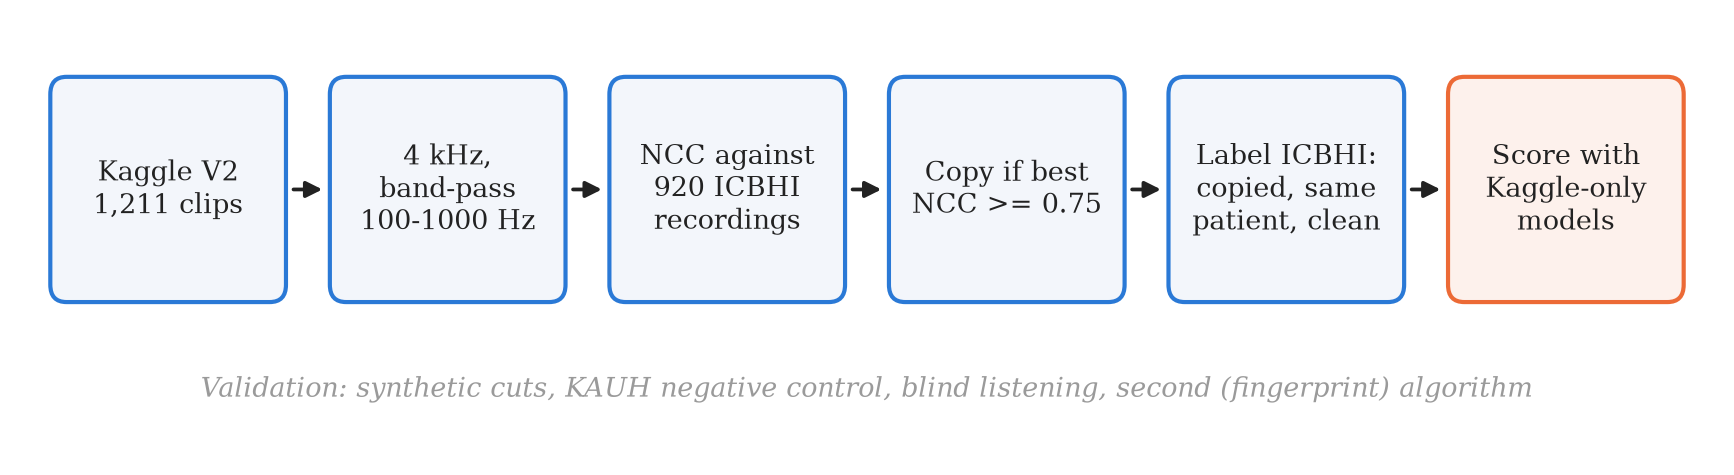
\includegraphics[width=0.92\textwidth]{figures/fig_pipeline.png}
    \caption{Audit pipeline: clip-to-recording matching, copy decision, and grouping of ICBHI recordings for the evaluation experiments.}
    \label{fig:pipeline}
\end{figure*}

\subsection{Matching clips to recordings}
All signals were resampled to 4~kHz and band-pass filtered between 100 and 1{,}000~Hz (fourth-order Butterworth, zero phase). For a clip $c$ of $n$ samples and an ICBHI recording $r$, we computed the normalized cross-correlation at every lag $\tau$:
\begin{equation}
\mathrm{NCC}(c,r,\tau)=\frac{\sum_{t=1}^{n}(c_t-\bar c)(r_{t+\tau}-\bar r_\tau)}{\sqrt{\sum_{t=1}^{n}(c_t-\bar c)^2\sum_{t=1}^{n}(r_{t+\tau}-\bar r_\tau)^2}}
\end{equation}
where $\bar r_\tau$ is the mean of the window of $r$ starting at $\tau$. NCC does not depend on gain, so the volume normalization described for the corpus does not hide a match. We kept the score
\begin{equation}
s(c)=\max_{r,\tau}\,|\mathrm{NCC}(c,r,\tau)|,
\end{equation}
together with the matching recording, its offset and the second-best score. A clip is a copy if $s(c)\geq 0.75$. If a recording is shorter than the clip, the roles are exchanged. An ICBHI patient is \emph{affected} if any of that patient's recordings is the source of a copied clip.

The threshold lies in an empty gap of the observed scores (Fig.~\ref{fig:ncc}): the lowest copy scored 0.795 and the highest non-copy 0.697, and no clip fell between them.

\subsection{Validation of the matcher}
We checked the matcher in four ways (results in Table~\ref{tab:valid}). (i)~We cut 100 synthetic degraded segments from ICBHI recordings with known sources and counted how many were matched to their true source. (ii)~We matched KAUH recordings against ICBHI as a negative control. (iii)~One of the authors listened blind to the 20 hardest real cases, the 10 lowest-scoring matches and the 10 highest-scoring non-matches, and judged whether each pair was the same audio. (iv)~A second algorithm based on landmark fingerprints, using the same 100--1{,}000~Hz band, was run on the same clips. It is a second algorithm, not an independent one.

\subsection{Effect on an ICBHI evaluation}
To measure what the copies do to an ICBHI test, we trained a single RespiNet-Attention v3 network (no ensemble, no fusion) from scratch on Kaggle data only, in two configurations: with all clips, and without the 631 ICBHI-derived clips. After removal of 12 byte-identical duplicates, the first configuration has 1{,}199 clips in five classes. The second has 568 clips in four classes: it has no COPD class, because every COPD clip is a copy. The corpus has no patient field, so we grouped clips by the number in the file name within each class folder; the 316 clips cut from KAUH recordings instead took the real KAUH patient identifier (40 patients in place of 64 file-name groups). Groups were split 60/20/20 for training, validation and test, stratified by class: 184 groups (110/37/37) with all clips and 97 (57/20/20) without the copies, giving 715 and 338 training recordings. Each configuration was trained with two seeds (42 and 43). The two seed-42 models were trained at an earlier code revision than the seed-43 models; only the later revision guarantees that the saved model is the one restored by early stopping, and the remaining differences concern code that a single network does not run. Seed 43 gives the same direction of effect (Section~IV-C).

All 920 ICBHI recordings were scored through the same prediction path as the served model: windows of 200 feature frames with a hop of 100, the mean of the window probabilities, and the top class, with no abstention. Each recording took its label from the patient's diagnosis: COPD, healthy, pneumonia and asthma map to the classes of the same name, and URTI, bronchiectasis, bronchiolitis and LRTI map to bronchial. Every recording was assigned to one of three groups: a \emph{copied recording} (the source of at least one Kaggle clip), a \emph{copied patient} (another recording of the same patient was copied), or \emph{clean} (the patient contributed nothing to the corpus).
% Release note (not for the text): model_metadata.json reports cross_dataset_overlap_exclusion: true for all four
% runs because that is the default setting; dataset_audit.json shows applied: false (all clips) and applied: true
% (631 removed, without copies). State this in the research release.

Two comparisons follow. In the \emph{within-model} design, one model trained with all clips is scored on copied versus clean recordings of the same class. In the \emph{between-model} design, the same copied recordings are scored by the model trained with the copies and by the one trained without. Because the second model has no COPD output, the between-model design covers bronchial, healthy and pneumonia only, and COPD enters the within-model design only. The first design compares different patients; the second holds the recordings fixed but changes the class set and training size.

\subsection{Statistics}
Accuracy is computed per recording. The difference between two accuracies is
\begin{equation}
\Delta=\mathrm{Acc}_A-\mathrm{Acc}_B,
\end{equation}
and its 95\% interval comes from a patient-cluster bootstrap with 10{,}000 draws, so recordings of one patient are resampled together. The listening check is summarised with an exact binomial interval.

\section{Result and analysis}
\subsection{How much of the corpus is derived from ICBHI}
Of 1{,}211 clips, 631 (52.1\%) are verbatim cuts of 187 ICBHI recordings belonging to 60 of the 126 ICBHI participants (Table~\ref{tab:prov}, Fig.~\ref{fig:prov}). All 401 COPD clips are ICBHI cuts. So are 105 of 285 pneumonia, 74 of 133 healthy and 51 of 104 bronchial clips. None of the 288 asthma clips is an ICBHI cut, but 262 of them are cuts of KAUH recordings. In total 316 clips are cut from 115 KAUH recordings, and 264 clips have no traced origin. The clips are therefore not independent samples: one ICBHI recording can be the source of several clips with different file-name identifiers.

\begin{table}
    \centering
    \captionsetup{justification=centering}
    \caption{Provenance of the 1{,}211 Kaggle clips by class (NCC $\geq$ 0.75)}
    \begin{tabular}{l|cccc}
        \hline
        \hline
        Class & Clips & ICBHI cuts & KAUH cuts & Untraced \\
        \hline
        Asthma    & 288 & 0   & 262 & 26  \\
        Bronchial & 104 & 51  & 15  & 38  \\
        COPD      & 401 & 401 & 0   & 0   \\
        Healthy   & 133 & 74  & 0   & 59  \\
        Pneumonia & 285 & 105 & 39  & 141 \\
        \hline
        \textbf{Total} & \textbf{1{,}211} & \textbf{631} & \textbf{316} & \textbf{264} \\
        \hline
        \hline
    \end{tabular}
    \label{tab:prov}
\end{table}

\begin{figure}
    \centering
    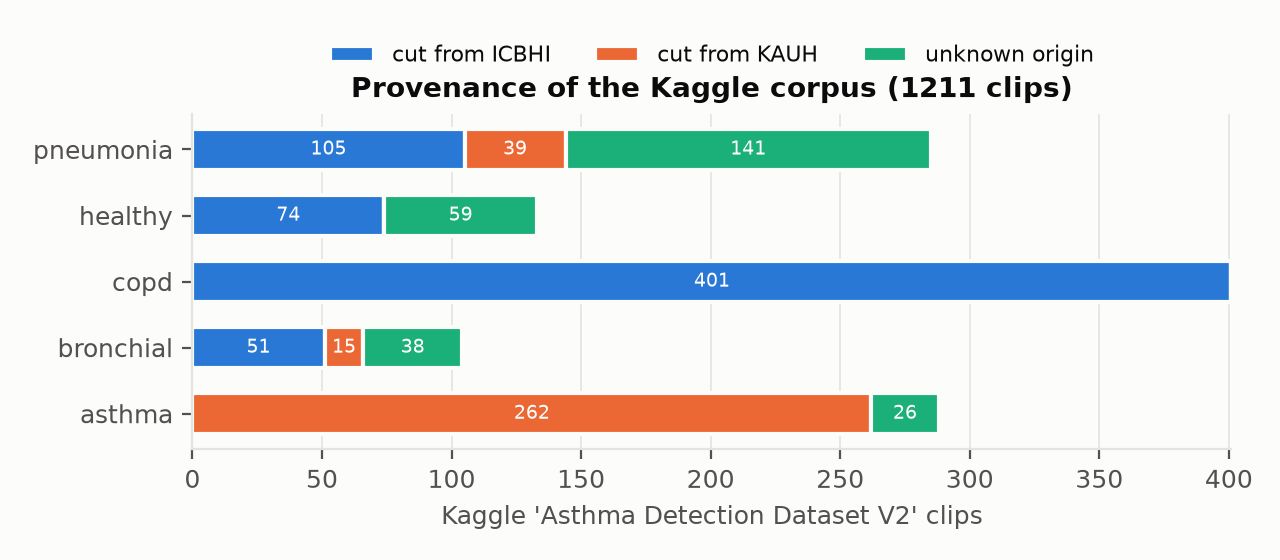
\includegraphics[width=\linewidth]{figures/fig1_overlap_by_class.png}
    \caption{Origin of the Kaggle clips by class. All COPD clips are ICBHI cuts; asthma clips are mostly KAUH cuts.}
    \label{fig:prov}
\end{figure}

\begin{figure}
    \centering
    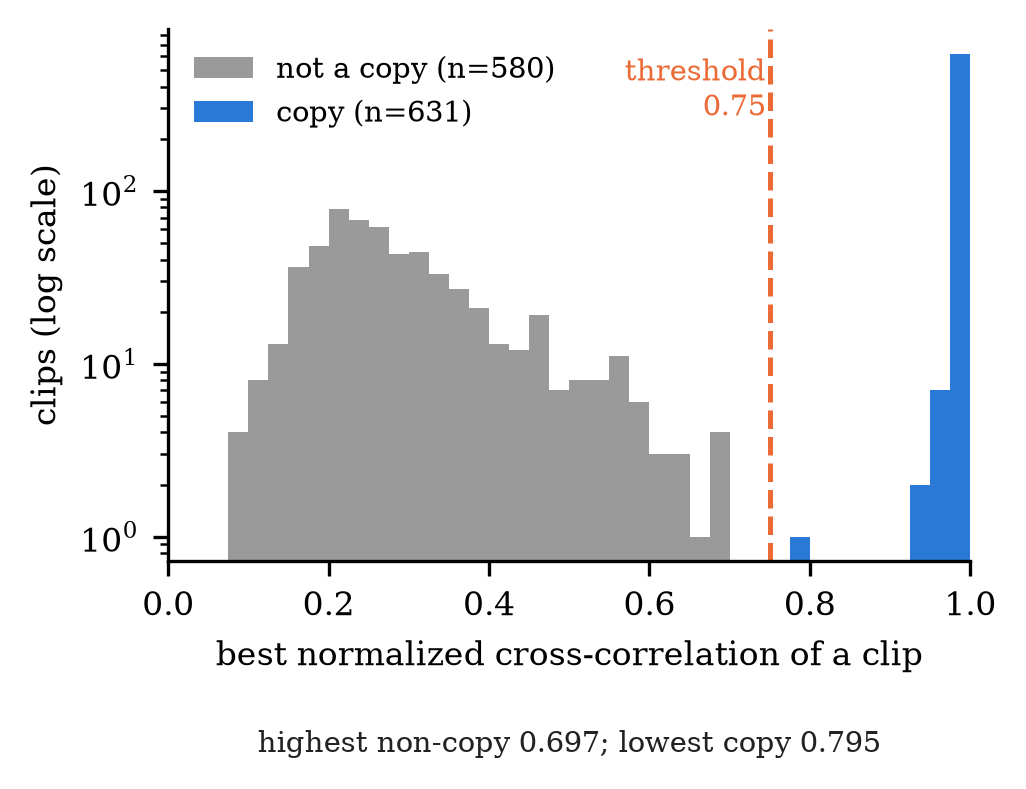
\includegraphics[width=0.95\linewidth]{figures/fig_ncc_hist.png}
    \caption{Best normalized cross-correlation of each Kaggle clip (log scale). No clip scores between 0.697 and 0.795; the threshold is 0.75.}
    \label{fig:ncc}
\end{figure}

\subsection{Validation of the matcher}
The scores separate cleanly (Fig.~\ref{fig:ncc}). Table~\ref{tab:valid} lists the validation results. Of 100 synthetic cuts, 99 were matched to their true source; the one miss scored 0.621, below the threshold, so our counts are lower bounds. No KAUH recording matched an ICBHI recording. In the blind listening check 19 of the 20 hardest cases were decided and all 19 agreed with the matcher (exact 95\% CI 82.4--100\%); one non-match was judged unsure. This check had a single rater, an author, so it supports the matcher without giving an error rate. The fingerprint algorithm found all 631 copies with the same source recordings and none additional, and 313 of the 316 KAUH-derived clips (the three it missed are clips of 0.7~s or less). Its synthetic recall was lower, 93 of 100.

\begin{table}
    \centering
    \captionsetup{justification=centering}
    \caption{Validation of the copy detector}
    \begin{tabular}{l|c}
        \hline
        \hline
        Check & Result \\
        \hline
        Synthetic degraded cuts, true source found & 99 / 100 \\
        KAUH recordings matching ICBHI & 0 \\
        Blind listening, 20 hardest cases & 19 / 19 agree \\
        Fingerprint algorithm, ICBHI copies & 631 / 631 \\
        Fingerprint algorithm, KAUH clips & 313 / 316 \\
        Fingerprint algorithm, extra matches & 0 \\
        Fingerprint algorithm, synthetic recall & 93 / 100 \\
        \hline
        \hline
    \end{tabular}
    \label{tab:valid}
\end{table}

\subsection{What the copies do to an ICBHI evaluation}
Within one model trained with all clips, copied ICBHI recordings were classified far more accurately than clean ones of the same class (Table~\ref{tab:effect}, Fig.~\ref{fig:effect}, left). For COPD, accuracy was 81.1\% on copied recordings (26 patients) against 41.5\% on clean ones (38 patients), a difference of $+39.5$ points (95\% CI 26.9 to 50.9). For bronchial sounds it was 62.5\% (7 patients) against 13.2\% (22 patients), $+49.3$ (23.4 to 82.1). With the second seed the differences were $+51.4$ (38.9 to 63.6) for COPD and $+65.5$ (32.0 to 85.4) for bronchial.

The between-model design keeps the recordings fixed (Fig.~\ref{fig:effect}, right). Removing the copies from training reduced accuracy on the copied healthy recordings from 96.2\% to 15.4\% (21 patients; $+80.8$, 65.4 to 93.6) and on the copied pneumonia recordings from 85.3\% to 32.4\% (6 patients; 27.3 to 71.4). For bronchial sounds the drop from 62.5\% to 43.8\% (7 patients) has an interval from $-25.0$ to $+61.5$ points, so this design is inconclusive for that class. The second seed shows the same direction for healthy (92.3\% to 34.6\%) and pneumonia (94.1\% to 38.2\%).

\begin{figure*}[t]
    \centering
    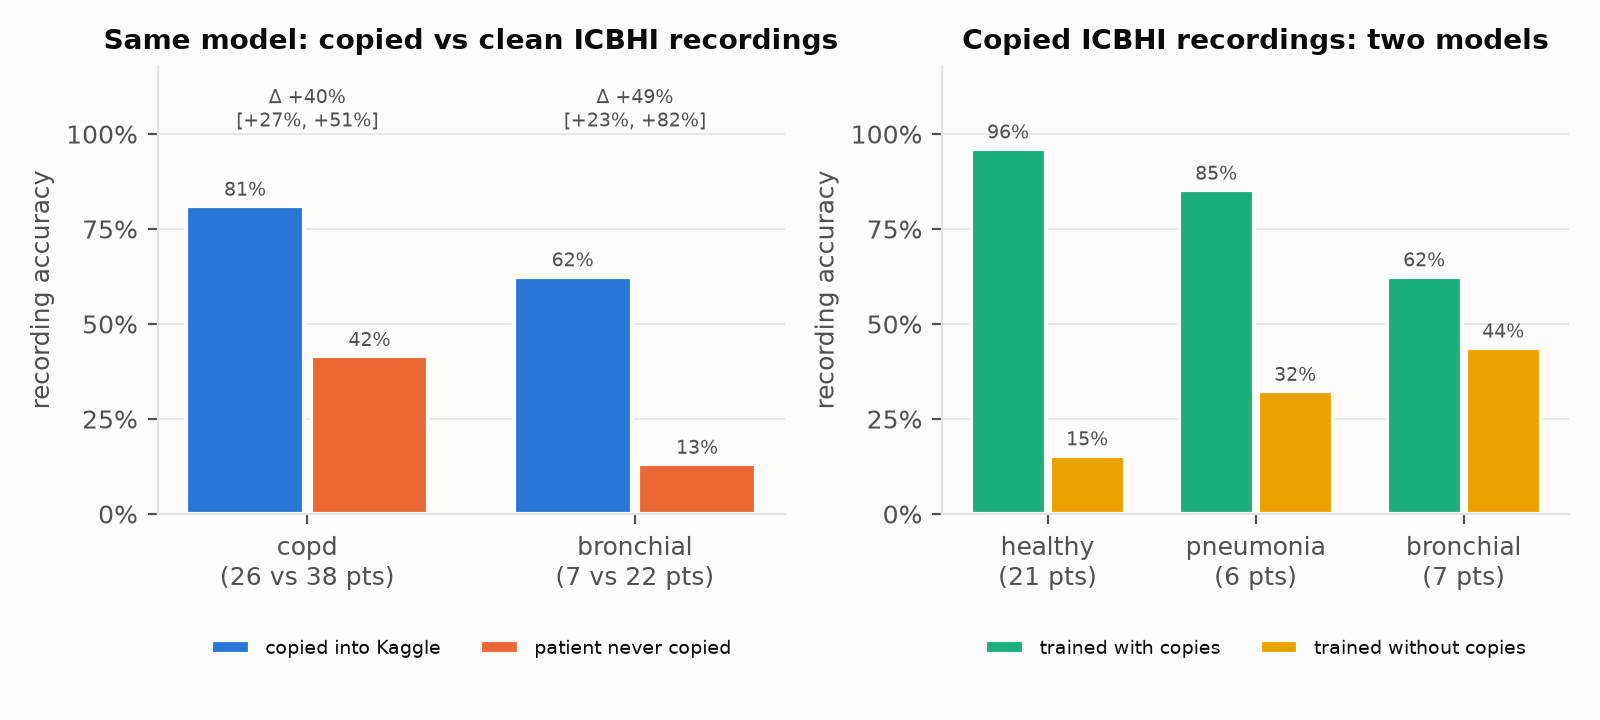
\includegraphics[width=0.85\textwidth]{figures/fig2_copied_vs_clean.png}
    \caption{Left: one Kaggle-trained model (copies in training) scored on copied versus clean ICBHI recordings of the same class; $\Delta$ with 95\% CI above the bars. Right: the same copied recordings scored by models trained with and without the copies. Seed 42; recording-level accuracy; patient counts under each class. The right panel has no COPD because the model without copies has no COPD class.}
    \label{fig:effect}
\end{figure*}

\begin{table}
    \centering
    \captionsetup{justification=centering}
    \caption{Accuracy contrasts on ICBHI recordings (seed 42; 95\% patient-cluster bootstrap CI)}
    \setlength{\tabcolsep}{3pt}
    \begin{tabular}{l|lcrr}
        \hline
        \hline
        Design & Class & Patients & Acc.\ (\%) & $\Delta$ [95\% CI] \\
        \hline
        Within-model & COPD      & 26/38 & 81.1 vs 41.5 & $+39.5$ [26.9, 50.9] \\
        (copied vs clean) & Bronchial & 7/22 & 62.5 vs 13.2 & $+49.3$ [23.4, 82.1] \\
        \hline
        Between-model & Healthy   & 21 & 96.2 vs 15.4 & $+80.8$ [65.4, 93.6] \\
        (with vs without & Pneumonia & 6 & 85.3 vs 32.4 & $+52.9$ [27.3, 71.4] \\
        copies) & Bronchial & 7 & 62.5 vs 43.8 & $+18.8$ [$-25.0$, 61.5] \\
        \hline
        \hline
    \end{tabular}
    \label{tab:effect}
\end{table}

\subsection{Interpretation}
The two designs ask different questions and have different weaknesses. The within-model design compares different patients, so copied recordings may simply be easier or may have been chosen by the uploader. The between-model design holds the recordings fixed, so recording difficulty cannot explain the drop; but removing the copies also removes the COPD class and shrinks the training set, so the drop cannot be assigned to contamination alone. If the copied recordings were merely easy, a model trained without the copies would still score them highly. The large drops for healthy and pneumonia therefore speak against that explanation, whereas the within-model gap alone cannot, since easier or selected recordings would produce it too. We nevertheless report the effect as an association, because neither design isolates the copies as a cause. The bronchial result is inconclusive in the between-model design and we draw no inference from it.

\subsection{Practical consequence}
A train-on-Kaggle, test-on-ICBHI evaluation partly re-tests training audio. Of the 920 ICBHI recordings, 187 were copied, and 310 more (304 of them COPD) belong to 29 of the 60 affected patients; the other 31 affected patients had every recording copied. The remaining 423 recordings come from the 66 clean patients. A cleaner evaluation excludes the copied recordings and the patients they belong to, which leaves at most these 423 recordings and 66 patients. Both are upper bounds, because 264 Kaggle clips have no traced origin.

The same check matters for KAUH. Because 262 of the 288 asthma clips are cuts of KAUH recordings, a cross-dataset test between the corpus and KAUH, which one study treats as independent \cite{tawfik2025erespinet}, is likely to re-test same-hospital, and possibly the same, audio on its asthma side. Its COPD side is a genuine cross-site comparison, since no COPD clip comes from KAUH. We did not re-run that study.

We suggest three steps before any split: (1) cross-match clips against the other public corpora in use; (2) report results separately for copied and clean material; (3) exclude copied recordings and their patients from any claimed external test.

\subsection{Limitations}
Counts are lower bounds, because the matcher missed one synthetic cut and was run at a single threshold; we did not run a threshold sweep. The listening check had one rater, an author. The compared groups contain different patients, uploader selection cannot be excluded, and the between-model design changes the class set and training size. Only two seeds were run, some classes have few patients (6 for pneumonia, 7 for bronchial), and accuracy is at recording level. We did not measure inflation on random or merged splits inside the corpus, and we did not re-run the setting of any published study, so we make no claim about the size of the error in published numbers.

\section{Conclusion and future work}
More than half of the Kaggle Asthma Detection Dataset V2 (631 of 1{,}211 clips) is cut from ICBHI recordings, including all COPD clips, and a Kaggle-trained model scores far higher on the ICBHI recordings that were copied than on clean ones. ICBHI is therefore not an independent external test for Kaggle-trained models unless the copied recordings and their patients are excluded. The corpus description does name ICBHI as a source; the new information is the extent, the class pattern and the structure of the overlap, which users need in order to build leak-free splits.

% CUT 2026-11-02 (outside the audit argument; small samples). To restore, cite the research release with a DOI
% and phrase it as exploratory:
% In separate analyses outside the scope of this paper, a model trained without KAUH healthy or COPD patients
% classified 0 of 45 external KAUH patients correctly, and a later model reached a balanced accuracy of 0.19 on an
% independent paediatric set; these concern different designs and are not part of the evidence above.

Before submission we plan to run a threshold sweep with pass/fail criteria fixed beforehand, add a second blind listener, and re-run the setting of the closest published study with and without the overlap. Inflation on merged or random splits inside the corpus remains future work.

\section*{Data availability, ethics, funding and AI use}
\textbf{Data.} ICBHI \cite{rocha2019} is freely available to the research community, with citation of \cite{rocha2019} requested; we found no named licence. KAUH \cite{fraiwan2021data} is released under CC BY 4.0, and the Kaggle corpus \cite{kaggleasthmav2} is listed under the Open Database and Database Contents licences, a label that does not change the terms of the ICBHI and KAUH audio it contains. We release no audio: the clip-to-recording match list holds only file names, offsets and match scores and, with the audit code, is available from the corresponding author on request. % VERIFY: ICBHI licence still not named (challenge site certificate expired; ask the maintainers). Reconfirm the Kaggle label with `kaggle datasets metadata mohammedtawfikmusaed/asthma-detection-dataset-version-2` before replacing "on request" with a repository link.
\textbf{Ethics.} No new human-subjects data were collected; all data are from public datasets used under their licences. \textbf{Funding and interests.} The authors received no funding and declare no conflict of interest. \textbf{Author contributions.} % VERIFY: CRediT roles for each author. Not invented.
\textbf{Use of AI tools.} AI tools (Claude and Copilot) were used for code assistance, literature-search support, and drafting and editing of text. The authors take responsibility for the content and checked every number against the evidence files.

%%BIB-START (generated by build_bibliography.py; do not edit by hand)
\begin{thebibliography}{00}
\bibitem{rocha2019} B. M. Rocha \textit{et al.}, ``An open access database for the evaluation of respiratory sound classification algorithms,'' \textit{Physiological Measurement}, vol. 40, no. 3, Art. no. 035001, 2019, doi: 10.1088/1361-6579/ab03ea.
\bibitem{fraiwan2021data} M. Fraiwan, L. Fraiwan, B. Khassawneh, and A. Ibnian, ``A dataset of lung sounds recorded from the chest wall using an electronic stethoscope,'' \textit{Data in Brief}, vol. 35, Art. no. 106913, 2021, doi: 10.1016/j.dib.2021.106913.
\bibitem{kaggleasthmav2} M. T. Musaed, ``Asthma Detection Dataset Version 2,'' Kaggle. Accessed 2026-11-01. [Online]. Available: \url{https://www.kaggle.com/datasets/mohammedtawfikmusaed/asthma-detection-dataset-version-2}
\bibitem{tawfik2022} M. Tawfik, N. M. Al-Zidi, I. Fathail, and S. Nimbhore, ``Asthma Detection System: Machine and Deep Learning-Based Techniques,'' in \textit{Artificial Intelligence and Sustainable Computing}. Springer, Singapore, 2022, pp. 207--218, doi: 10.1007/978-981-19-1653-3\_16.
\bibitem{shatat2026} G. A. E.-L. Shatat, H. E.-D. Moustafa, M. S. Saraya, A.-S. A. Marzouk, and A. A. Hekal, ``Hybrid deep learning and {YAMNet} features for asthma diagnosis from respiratory sounds,'' \textit{Scientific Reports}, vol. 16, Art. no. 13781, 2026, doi: 10.1038/s41598-026-49247-y.
\bibitem{tawfik2025erespinet} M. Tawfik, I. S. Fathi, S. S. Nimbhore, I. M. Alsmadi, and M. S. Sawah, ``{E-RespiNet}: An {LLM-ELECTRA} driven triple-stream {CNN} with feature fusion for asthma classification,'' \textit{PLoS ONE}, vol. 20, no. 11, Art. no. e0334528, 2025, doi: 10.1371/journal.pone.0334528.
\bibitem{saky2026} S. M. A. I. Saky \textit{et al.}, ``Explainable multi-modal deep learning for recording-level classification of respiratory audio signals under internal and domain-shift evaluation,'' \textit{Life}, vol. 16, no. 7, Art. no. 1108, 2026, doi: 10.3390/life16071108.
\bibitem{topaloglu2025} I. Topaloglu \textit{et al.}, ``Machine learning-driven lung sound analysis: Novel methodology for asthma diagnosis,'' \textit{Advances in Respiratory Medicine}, vol. 93, no. 5, Art. no. 32, 2025, doi: 10.3390/arm93050032.
\bibitem{dolu2026} K. O. Dolu, ``Comment on {Topaloglu et al.} Machine learning-driven lung sound analysis: Novel methodology for asthma diagnosis,'' \textit{Advances in Respiratory Medicine}, vol. 94, no. 2, Art. no. 15, 2026, doi: 10.3390/arm94020015.
\bibitem{pham2021} L. Pham, H. Phan, R. Palaniappan, A. Mertins, and I. McLoughlin, ``{CNN-MoE} based framework for classification of respiratory anomalies and lung disease detection,'' \textit{IEEE Journal of Biomedical and Health Informatics}, vol. 25, no. 8, pp. 2938--2947, 2021, doi: 10.1109/JBHI.2021.3064237.
\bibitem{nguyen2022} T. Nguyen and F. Pernkopf, ``Lung sound classification using co-tuning and stochastic normalization,'' \textit{IEEE Transactions on Biomedical Engineering}, vol. 69, no. 9, pp. 2872--2882, 2022, doi: 10.1109/TBME.2022.3156293.
\bibitem{pessoa2026} D. Pessoa, J. Garcia, J. De La Torre-Cruz, F. Ca{\~n}adas-Quesada, and R. P. Paiva, ``Automated diagnosis of respiratory diseases from respiratory sounds: A reproducibility case study,'' in \textit{Proc. 19th Int. Joint Conf. Biomedical Engineering Systems and Technologies (BIOSIGNALS)}, 2026, pp. 392--397, doi: 10.5220/0014430000004070.
\bibitem{onglyi2024} C. Ong Ly \textit{et al.}, ``Shortcut learning in medical {AI} hinders generalization: method for estimating {AI} model generalization without external data,'' \textit{npj Digital Medicine}, vol. 7, Art. no. 124, 2024, doi: 10.1038/s41746-024-01118-4.
\bibitem{kapoor2023} S. Kapoor and A. Narayanan, ``Leakage and the reproducibility crisis in machine-learning-based science,'' \textit{Patterns}, vol. 4, no. 9, Art. no. 100804, 2023, doi: 10.1016/j.patter.2023.100804.
\bibitem{abhishek2025} K. Abhishek, A. Jain, and G. Hamarneh, ``Investigating the quality of {DermaMNIST} and {Fitzpatrick17k} dermatological image datasets,'' \textit{Scientific Data}, vol. 12, Art. no. 196, 2025, doi: 10.1038/s41597-025-04382-5.
\bibitem{kim2024} J.-W. Kim, S. Bae, W.-Y. Cho, B. Lee, and H.-Y. Jung, ``Stethoscope-guided supervised contrastive learning for cross-domain adaptation on respiratory sound classification,'' in \textit{Proc. IEEE Int. Conf. Acoustics, Speech and Signal Processing (ICASSP)}, 2024, pp. 1431--1435, doi: 10.1109/ICASSP48485.2024.10447734.
\bibitem{zech2018} J. R. Zech, M. A. Badgeley, M. Liu, A. B. Costa, J. J. Titano, and E. K. Oermann, ``Variable generalization performance of a deep learning model to detect pneumonia in chest radiographs: A cross-sectional study,'' \textit{PLOS Medicine}, vol. 15, no. 11, Art. no. e1002683, 2018, doi: 10.1371/journal.pmed.1002683.
\bibitem{jimenez2024} A. Jim{\'e}nez-S{\'a}nchez \textit{et al.}, ``Copycats: the many lives of a publicly available medical imaging dataset,'' in \textit{Advances in Neural Information Processing Systems (Datasets and Benchmarks Track)}, vol. 37, 2024, pp. 113383--113404, doi: 10.52202/079017-3602.
\end{thebibliography}
%%BIB-END

\end{document}
